\documentclass{article}
\usepackage[dvipsnames]{xcolor}
\usepackage{tikz}

\tikzstyle{vertex}=[circle, thick, draw=black, inner sep = 2pt]
\tikzstyle{positive}=[ultra thick, color=blue]
\tikzstyle{negative}=[ultra thick, color=red]

\begin{document}

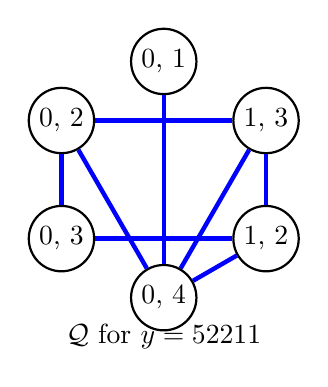
\begin{tikzpicture}[scale=.5]
\node[vertex] (0_1) at (90:3) {0, 1};
\node[vertex] (0_2) at (150:3) {0, 2};
\node[vertex] (0_3) at (210:3) {0, 3};
\node[vertex] (0_4) at (270:3) {0, 4};
\node[vertex] (1_2) at (330:3) {1, 2};
\node[vertex] (1_3) at (390:3) {1, 3};

\node at (270:4) {$\mathcal{Q}$ for $y = 5 2 2 1 1 $};
\draw[positive] (0_1)--(0_4);
\draw[positive] (0_2)--(0_3);
\draw[positive] (0_2)--(0_4);
\draw[positive] (0_2)--(1_3);
\draw[positive] (0_3)--(1_2);
\draw[positive] (0_4)--(1_2);
\draw[positive] (0_4)--(1_3);
\draw[positive] (1_2)--(1_3);
\end{tikzpicture}
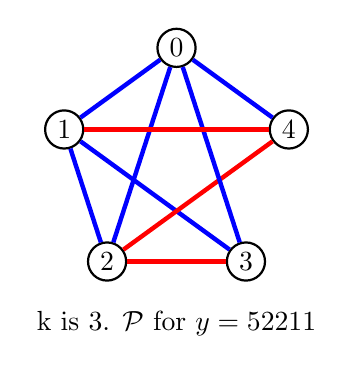
\begin{tikzpicture}[scale=.5]
\foreach \i in {0,1,2,...,4}
\node[vertex] (\i) at ({90 + 72*(\i)}:3){\i};

\node at (270:4) {k is 3. $\mathcal{P}$ for $y = 5 2 2 1 1 $};
\draw[positive] (0)--(1);
\draw[positive] (1)--(2);
\draw[negative] (2)--(3);
\draw[positive] (0)--(2);
\draw[positive] (1)--(3);
\draw[negative] (2)--(4);
\draw[positive] (0)--(3);
\draw[negative] (1)--(4);
\draw[positive] (0)--(4);
\end{tikzpicture}
\end{document}
